\section{$\mathit{plus1}$}

\subsection{\texttt{Plus1.hs}}
ForSyDe specification model of a simple adder system.
 
\lstinputlisting[language=haskell]{B.Examples/Plus1.hs}
\clearpage
\subsection{\texttt{plus1.vhd}}
VHDL code generated from its Haskell model. Note that the code depends
on ForSyDe's VHDL Library, which is included in appendix
\ref{chap:vhdllib}.

\lstinputlisting[language=VHDL]{B.Examples/plus1.vhd}
\newpage
\subsection{RTL model of $\mathit{plus1}$}
RTL model obtained with Altera's \textit{Quartus II} software after
compiling the VHDL model for a Stratix FPGA.

\begin{figure}[h]
\centering
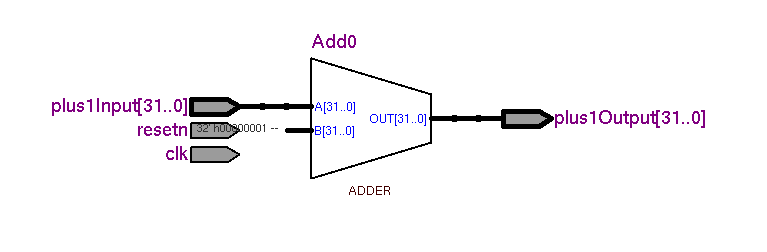
\includegraphics[scale=.7]{plus1.png}
\caption{RTL model of $\mathit{plus1}$}
\end{figure}
